\subsection{Background on point processes}\label{background_tpp}

In this section, we will give a short introduction on point processes, and particularly on temporal point processes with a focus on Hawkes processes.
Further details can be found in \citep{daley2003introduction, daley2007introduction}.
The sub-section~\ref{pp_definitions} comes from the PhD thesis of Massil Achab~\citep{achab2017learning}.

\subsubsection{Definitions}\label{pp_definitions}
A point process is a random element whose values are point patterns on a set $S$, a locally compact metric space equipped with its Borel $\sigma$-algebra $\mathscr{B}$.
Let $X_S$ be the set of locally finite counting measures on $S$, and $\mathcal{N}_S$ the smallest $\sigma$-algebra on $X_S$ such that all point counts ${f_B: X_s \to \N, \omega \mapsto \#\pars{\omega \cap B}}$ are measurable for $B$ relatively compact in $\mathscr{B}$, where $\# A$ denotes the cardinality of the set $A$.
A point process on $S$ is a measurable map $\xi$ from a probability space $\pars{\Omega, \mathcal{F}, \proba{}}$ to the measurable space $\pars{X_S, \mathcal{N}_S}$.

Every realisation of a point process $\xi$ can be written as $\xi = \sum_{i=1}^n \dirac_{X_i}$, where $\dirac$ is the Dirac measure, $n$ is an integer-valued random variable and $X_i$'s are random elements of $S$.
A point process can be equivalently represented by a counting process $N\pars{B} \coloneqq \integ{B}{\xi (x)}{x}$ which basically is the number of event in each Borel subset $B\in\mathscr{B}$.
The mean measure $M$ of a point process $\xi$ is a measure on $S$ that assigns to every $B\in\mathscr{B}$ the expected number of event of $\xi$ in $B$, i.e., $M\pars{B} \coloneqq \esp{N\pars{B}}$ for all $B\in\mathscr{B}$.


\subsubsection{Temporal point processes}
A temporal point process is a stochastic, or random, process composed of a time series of binary events that occur in continuous time\footnote{\href{http://www.stat.columbia.edu/~liam/teaching/neurostat-fall19/uri-eden-point-process-notes.pdf}{Liam Paninski, Statistical analysis of neural data, Fall 2019, \textit{Chapter 2: Introduction to Point Processes} - Columbia Statistics}}.
However, on the contrary of time series, temporal point processes can study multiple time scales at once~\citep{bompaire2019machine}. 

In this particular case, $S$ is the time interval $\intervalleFO{0}{T}$, equipped with the Borel $\sigma$-field of the real line $\mathscr{B}\pars{\R}$.
Here, a realisation of a point process is simply a set of time points: $\xi = \sum_{i=1}^n \delta_{t_i}$.
With a slight abuse of notation, we associate to the set of distinct random timestamps $\xi = \braces{t_1, \dots, t_n}$ occurring before $T$, the counting process $N_t = \sum_{t_i \in\xi}\1[t_i \leq t]$, which is then simply the number of points in the time interval $\intervalleOF{0}{t}$.
This counting process is a random process which evolves over time by jumps of size 1.
Studying temporal point processes consists in analysing when this jumps occur.
The \textit{conditional intensity} function $\lambda\pars{t \middle| \mathscr{F}_t}$ is the usual way to characterise temporal point processes where the present depends on the past.
It is defined as the expected infinitesimal rate at which events are expected to occur after $t$ given the information $\mathscr{F}_t$ available up to (but not including) time $t$, i.e., the history of the counting process $N_t$ prior to $t$.
Namely,
\begin{equation}
    \lambda\pars{t \middle| \mathscr{F}_t} = \lim_{\dint t \to 0} \frac{\proba{N_{t + \dint t} - N_t = 1}[\mathscr{F}_t]}{\dint t}
\end{equation}
where $\mathscr{F}_t = \enstq{t_i}{t_i < t, i=1,\dots,n}$ is the natural filtration of the process.
The conditional intensity function is sometimes denoted $\lambda^*(t)$.

As $\dint N_t \coloneqq N_{t +\dint t} - N_t \in \braces{0,1}$ can only increase by one event at each $\dint t$, it readily follows that $\proba{\dint N_t = 1}[\mathscr{F}_t] = \lambda^*(t)\dint t$ and
\begin{equation}
    \esp{\dint N_t}[\mathscr{F}_t] = 1\times \proba{\dint N_t = 1}[\mathscr{F}_t] + 0\times \proba{\dint N_t = 0}[\mathscr{F}_t] = \lambda^*(t)\dint t
\end{equation}
Hence, we can also think of the conditional intensity function $\lambda^*(t)$ as an instantaneous rate of events per time of unit.

The \textit{homogeneous Poisson process} is the most simple temporal point process, which assumes that the events arrive at a constant rate, which corresponds to a constant intensity function $\lambda\pars{t \middle| \mathscr{F}_t} = \lambda^*(t) = \lambda > 0$.
In other words, it describes a phenomenon with no memory and a constant probability of occurrence in which $N_{t + \Delta t} - N_t$ follows a Poisson distribution of parameter $\Delta t$ for any $\Delta t > 0$.
For this process, $\forall B \in \mathscr{B}\pars{\R}, M\pars{B} = \lambda \abs{B}$, where $\abs{\cdot}$ is the Lebesgue measure on $\pars{S, \mathscr{B}\pars{\R}}$.

The \textit{inhomogeneous Poisson process} is a more general process, for which the conditional intensity function is not constant as it depends on $t$ but \textit{not} on the history, i.e. ${\lambda\pars{t \middle| \mathscr{F}_t} = \lambda^*(t) = \lambda(t)}$.
For this process, $M\pars{B} = \integ{B}{\lambda(x)}{x}$, for all $B \in \mathscr{B}\pars{\R}$.

Let us denote $f^*(t) = f\pars{t \middle| \mathscr{F}_t}$ the conditional probability density function of the inter-event time, i.e., the probability that the next event will occur during the interval $\intervalleFO{t}{t+\dint t}$ conditioned on the history $\mathscr{F}_t$.
Let us also denote $F^*(t) = F\pars{t \middle| \mathscr{F}_t} = \proba{t_n \leq t_{n+1} \leq t}[\mathscr{F}_t] =  \integ{t_{n}}[t]{f^*(\tau)}{\tau}$ the conditional cumulative density function, i.e., the probability that the next event will occur before time $t$ conditioned on the history $\mathscr{F}_t$, where here $t_n$ is the last event in $\mathscr{F}_t$, i.e., the last event before time $t$.
Finally, we denote $S^*(t) = 1 - F^*(t) = \proba{t_{n+1} \geq t}[\mathscr{F}_t]$ the complementary cumulative distribution, also called the survival function, i.e., the probability that the next event will not occur before time $t$ conditioned on the history $\mathscr{F}_t$ \citep{de2019temporal}.
Now,
\begin{equation}
    \begin{split}
        \lambda^*(t) &= \lim_{\dint t \to 0} \frac{\proba{t\leq t_{n+1} \leq t+\dint t}[t_{n+1} > t]}{\dint t} \\
        &= \lim_{\dint t \to 0} \frac{1}{\dint t} \frac{\proba{t\leq t_{n+1} \leq t+\dint t}}{\proba{t_{n+1} > t}} \\
        &= \lim_{\dint t \to 0} \pars{\frac{1}{\dint t}\frac{f^*(t)\dint t}{S^*(t)} + o(1)} \\
        &= \frac{f^*(t)}{S^*(t)} \\
        &= - \frac{1}{S^*(t)} \deriv{S^*(t)}{t} \\
        &= -\deriv{\log S^*(t)}{t}
    \end{split}
\end{equation}
By integrating the left and right hand sides in the above equation, we have that
\begin{equation}
    \integ{t_n}[t]{\lambda^*(\tau)}{\tau} = \integ{t_n}[t]{-\deriv{\log S^*(\tau)}{\tau}}{\tau} = -\log S^*(t) + \underbrace{\log S^*(t_n)}_{=0}
\end{equation}
and thus,
\begin{equation}
    S^*(t) = \e{- \integ{t_n}[t]{\lambda^*(\tau)}{\tau}}
\end{equation}
Finally, we get that
\begin{equation}\label{eq:f_star_res}
    f^*(t) = \lambda^*(t) \e{- \integ{t_n}[t]{\lambda^*(\tau)}{\tau}}
\end{equation}

\subsubsection{Poisson process and likelihood function}

This section is taken and adapted from \citep[chap.~2, p.~19-23]{daley2003introduction} and aims to give a more in-depth presentation of the Poisson processes, with a focus on the computation of the likelihood function, as it is a crucial information for the report.

The stationary Poisson process\footnote{What we previously called the homogeneous Poisson process.}, on the line is completely defined by the following equation, in which we use $N\intervalleOF{a_i}{b_i}$ to denote the number of events of the process falling in the half-open interval $\intervalleOF{a_i}{b_i}$ with $a_i < b_i \leq a_i+1$:
\begin{equation}\label{eq:def_stationary_pp}
    \proba{N\intervalleOF{a_i}{b_i} = n_i, i=1,\dots,k} = \prod_{i=1}^k \frac{\bracks{\lambda\pars{b_i-a_i}}^{n_i}}{n_i!}e^{-\lambda\pars{b_i-a_i}}
\end{equation}

This definition embodies three important features:
\begin{itemize}
    \item the number of points in each finite interval $\intervalleOF{a_i}{b_i}$ has a Poisson distribution of parameter~$\lambda$;
    
    \item the numbers of points in disjoint intervals are independent random variables; and
    
    \item the distributions are stationary: they depend only on the lengths $b_i - a_i$ of the intervals.
\end{itemize}

The likelihood of a finite realisation of a Poisson process may be defined as the probability of obtaining the given number of observations in the observation period, times the joint conditional density for the positions of those observations, given their number.

Suppose that there are $N$ observations on $\intervalleOF{0}{T}$ at time points $t_1,\dots,t_N$. From \ref{eq:def_stationary_pp}, we can write down immediately the probability of obtaining single events in $\intervalleOF{t_i-\Delta}{t_i}$ and no points on the remaining part of $\intervalleOF{0}{T}$.
Let $A$ and $B$ be respectively those events, namely, 
$$A = \braces{N\intervalleOF{t_i-\Delta}{t_i} = 1, i=1,\dots,N}$$
and
$$B = \braces{N\intervalleOF{0}{t_{1}-\Delta} = 0, N\intervalleOF{t_N}{T} = 0, N\intervalleOF{t_i}{t_{i+1}-\Delta} = 0, i=1,\dots,N-1}$$
\begin{align*}
    \proba{A\cap B} &= \prod_{i=1}^N \pars{\lambda\Delta e^{-\lambda\Delta}} \times e^{-\lambda\pars{t_1 - \Delta}} \times e^{-\lambda\pars{T-t_N}} \times \prod_{i=1}^{N-1} e^{-\lambda\pars{t_{i+1}-\Delta-t_i}} \\
    &= \prod_{i=1}^N \pars{\lambda\Delta} \times e^{-\lambda \Delta N} \times e^{-\lambda\pars{T-N\Delta}} \\
    &= e^{-\lambda T} \prod_{i=1}^N \lambda\Delta \\
    &= \lambda^N \Delta^N e^{-\lambda T}
\end{align*}

Dividing by $\Delta^N$ and letting $\Delta \xrightarrow{} 0$, to obtain the density, we find as the required likelihood function
\begin{equation}
    L_{\intervalleOF{0}{T}}\pars{N;t_1,\dots,t_n} = \lambda^N e^{-\lambda T}
\end{equation}

We can extend this result to a Poisson process with time-varying rate $\lambda(t)$, commonly called the \textit{nonhomogeneous} or \textit{inhomogeneous} Poisson process.
The process can be defined exactly as in \ref{eq:def_stationary_pp}, ,with the quantities $\lambda\intervalleOF{a_i}{b_i} = \integ{a_i}[b_i]{\lambda}{x}$ replaced wherever they occur by quantities
$$ \Lambda\intervalleOF{a_i}{b_i} = \integ{a_i}[b_i]{\lambda(x)}{x}$$
called the \textit{compensator} of the point process.
Thus, the joint distributions are still Poisson, and the independence property still holds.
The likelihood function takes the more general form
\begin{equation}\label{eq:general_likelihood}
\begin{split}
    L_{\intervalleOF{0}{T}}\pars{N;t_1,\dots,t_n} &= e^{-\Lambda\intervalleOF{0}{T}} \prod_{i=1}^N \lambda(t_i) \\
    &= \e{-\integ{0}[T]{\lambda(t)}{t} + \sum_{i=1}^N \log \lambda(t_i)} \\
    &= \e{-\integ{0}[T]{\lambda(t)}{t} + \int_0^T \log \lambda(t)N\pars{\dint t}}
\end{split}
\end{equation}

Note that this result could also be obtained by using the Equation~\eqref{eq:f_star_res}.

\subsubsection{Hawkes processes}\label{hawkes_processes}

In this section, we give the main definitions and properties of Hawkes processes and multivariate Hawkes processes and set the notations that will be used in the rest of the report.
Hawkes processes~\citep{hawkes1971point, hawkes1974cluster} are temporal point processes in which the intensity depends on the process history with an excitation mechanism.
They can be understood as the equivalent of auto-regressive time series models (AR) but in continuous time.
This allows to study cross causality that might occur in one or several events series~\citep{bompaire2019machine}.

An Hawkes process is thus defined by a history dependent intensity $\lambda$ defined as follows:
\begin{equation}\label{eq:uni_hawkes_process}
    \lambda\pars{t\middle| \mathscr{F}_t} = \psi\pars{\mu + \integ{-\infty}[t]{\phi(t-s)}{N_s}}
\end{equation}
where 
\begin{equation}
    \integ{-\infty}[t]{\phi(t-s)}{N_s} = \sum_{i, t_i<t} \phi(t-t_i)
\end{equation}
The $\mu \geq 0$ is referred as the \textit{baseline intensity}\footnote{Some authors may also call it the background intensity.} and it corresponds to the exogenous intensity of the considered events.
The function $\phi(\cdot):\R^+\to\R$ is called the \textit{kernel function}, or the transfer function~\citep{chen2017multivariate}, and quantifies over time and in magnitude the influence of past events.
Note that the occurrence of each event $t_i$ increases the intensity by a certain amount, determined by the kernel, making the intensity history dependent and a stochastic process by itself \citep{de2019temporal}.
If the \textit{link function} $\psi$ on the right-hand side of Eq.~\ref{eq:uni_hawkes_process} is non-linear, then $\lambda(t)$ is the intensity of a non-linear Hawkes process~\citep{bremaud1996stability}.
In what follows, we only consider the case where $\psi$ is the identity function.

\paragraph{Multivariate Hawkes process} We can extend the univariate Hawkes process to model the interactions of $K\geq 1$ temporal point processes, called \textit{nodes}.

Namely, it models timestamps $\braces{t_k^{(i)}}_{k\geq 1}$ of nodes $i=1,\dots,K$ associated with a multivariate counting process $N_t = \bracks{N_t^{(1)}, \dots, N_t^{(K)}}$.
Note that for all nodes $i=1,\dots,K$, we still have that all of its timestamps $t_k^{(i)}$ occur in the time interval $\intervalleFF{0}{T}$.
The excitation dynamic between the nodes is encompassed by the auto-regressive structure of the conditional intensity.
For component $N_t^{(i)}$ it writes
\begin{equation}
    \lambda_i\pars{t \middle| \mathscr{F}_t} = \mu_i + \sum_{j=1}^K  \integ{-\infty}[t]{\phi_{i,j}(t-s)}{N_s^{(j)}}
\end{equation}
where $\phi_{i,j}(t)$ quantifies the excitation rate of an event of type $j$ on the arrival rate of events of type $i$ after a time lag $t$.
In general it is assumed that each kernel is causal and positive, meaning that Hawkes processes can only account for mutual excitation effects since the occurrence of some event can only increase the future arrival intensity of other events.
If the kernels are integrable, each entry of the $K\times K$ matrix ${\pars{\Phi}_{i,j} = \integ{0}[T]{\phi_{i,j}(t)}{t}}$ denotes the expected number of events of type $i$ directly triggered by an event of type $j$.

\begin{figure}[h]
    \centering
    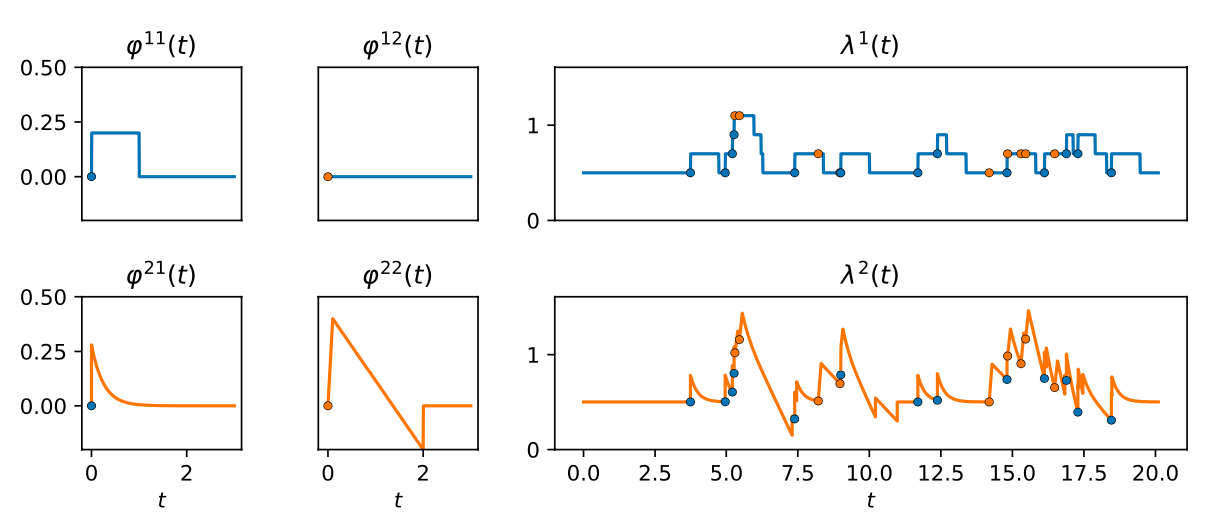
\includegraphics[scale=0.35]{pics/simu_multi_hawkes.png}
    \caption{A realisation of a 2 nodes multivariate Hawkes process using \texttt{Tick} package. The four excitation kernels are shown on the left hand side. The intensities are displayed on the right hand side (against time, up to time 20), where events are represented by coloured dots (blue corresponding to node 1 and orange to node 2).}
    \source{\citep{bompaire2019machine}}
    \label{fig:tick_hawkes_model}
\end{figure}

\paragraph{Kernels parametrisation}
The main parametric model is the so-called \textit{exponential kernel}, in which the kernels have the following form:
\begin{equation}
    \phi_{i,j}(t) = \alpha_{i,j} \beta \e{-\beta t}, \quad \alpha_{i,j} > 0, \beta > 0
\end{equation}
In this model the integral matrix $\Phi = \pars{\alpha_{i,j}}_{1\leq i,j\leq K}$ and $\beta > 0$ is a memory parameter.
A more general approach is the \textit{sum of exponentials kernels}~\citep{lemonnier2014nonparametric}, namely
\begin{equation}
    \phi_{i,j}(t) = \sum_{u=1}^U \alpha_{i,j}^{(u)} \beta^{(u)} \e{-\beta^{(u)} t}, \quad \alpha_{i,j}^{(u)} > 0, \beta^{(u)} > 0
\end{equation}

Similarly, we can define the \textit{gaussian kernel} and the \textit{sum of gaussians kernels}.
In python, the \texttt{Tick} package allows to easily manipulate Hawkes process with exponential and gaussian kernels~\citep{bompaire2019machine, bacry2017tick}.
Other kernel functions are presented in~\citep{mehrdad2014hawkes}.
